\NeedsTeXFormat{LaTeX2e}
\documentclass[a4paper,12pt,
headsepline,           % Linie zw. Kopfzeile und Text
twoside,               % zweiseitig
pointlessnumbers,      % keine Punkte nach den letzten Ziffern in Überschriften
bibtotoc,              % LV im IV
%DIV=15,               % Satzspiegel auf 15er Raster, schmalere Ränder   
BCOR15mm               % Bindekorrektur
%,draft
]{scrbook}
\KOMAoptions{DIV=last} % Neuberechnung Satzspiegel nach Laden von Paket helvet

\pagestyle{headings}
\usepackage{blindtext}

% für Texte in deutscher Sprache
\usepackage[ngerman]{babel}
\usepackage[utf8]{inputenc}
\usepackage[T1]{fontenc}

% Helvetica als Standard-Dokumentschrift
\usepackage[scaled]{helvet}
%\usepackage{mathptmx}
\renewcommand{\familydefault}{\sfdefault} 

\usepackage{graphicx}

% Für Tabellen mit fester Gesamtbreite und variabler Spaltenbreite
\usepackage{tabularx} 

% Besondere Schriftauszeichnungen
\usepackage{url}              % \url{http://...} in Schreibmaschinenschrift
\usepackage{color}            % zum Setzen farbigen Textes

\usepackage{amssymb, amsmath} % Pakete für Mathe-Umgebungen und -Symbole

\usepackage{setspace}         % Paket für div. Abstände, z.B. ZA
%\onehalfspacing              % nur dann, wenn gefordert; ist sehr groß!!
\setlength{\parindent}{0pt}   % kein linker Einzug der ersten Absatzzeile
\setlength{\parskip}{1.4ex plus 0.35ex minus 0.3ex} % Absatzabstand, leicht variabel

% Tiefe, bis zu der Überschriften in das Inhaltsverzeichnis kommen
\setcounter{tocdepth}{3}      % ist Standard


%\usepackage[printonlyused, withpage]{acronym}
\usepackage[printonlyused]{acronym}
\usepackage{comment}
\usepackage{longtable}
%\usepackage[maxdepth=8, mark]{gitinfo2}
\usepackage{bytefield}
\usepackage{smartdiagram}
\usepackage{caption}
\usepackage{hyperref}
\usepackage{hypcap}
\usepackage{graphicx}
\usepackage{tikz}
\usepackage{mathtools}
\usepackage{colortbl}
\usepackage{xcolor}
\usepackage[outline]{contour}
\usetikzlibrary{arrows}
\usetikzlibrary{calc,positioning,shapes,decorations.pathreplacing, matrix, backgrounds, fit}

% hier Namen etc. einsetzen
\newcommand{\fullname}{Björn Petersen}
\newcommand{\email}{bjoern.petersen@uni-ulm.de}
\newcommand{\titel}{Darstellung und Analyse SoC interner Kommunikationskanäle auf Protokollebene}
\newcommand{\jahr}{2020}
\newcommand{\matnr}{941984}
\newcommand{\gutachterA}{Prof.\,Dr.-Ing\,Maurits Ortmanns}
\newcommand{\gutachterB}{Dr.\,rer.\,nat.\,Dipl.-Ing\,Endric Schubert}
\newcommand{\betreuer}{Dipl-Ing\, Ulrich Langenbach}

% hier die Fakultät auswählen
%\newcommand{\fakultaet}{---  Im Quellcode anpassen nicht vergessen! ---}
\newcommand{\fakultaet}{Ingenieurwissenschaften, Informatik und\\Psychologie}
%\newcommand{\fakultaet}{Mathematik und\\Wirtschafts-\\wissenschaften}
%\newcommand{\fakultaet}{Medizin}
%\newcommand{\fakultaet}{Naturwissenschaften}

% hier das Institut einsetzen
\newcommand{\institut}{Institut für Mikroelektronik}

% Informationen, die LaTeX in die PDF-Datei schreibt
\pdfinfo{
  /Author (\fullname)
  /Title (\titel)
  /Producer     (pdfeTex 3.14159-1.30.6-2.2)
  /Keywords ()
}

\usepackage{hyperref}
\hypersetup{
pdftitle=\titel,
pdfauthor=\fullname,
pdfsubject={Diplomarbeit},
pdfproducer={pdfeTex 3.14159-1.30.6-2.2},
colorlinks=false,
pdfborder=0 0 0	% keine Box um die Links!
}

\usepackage{listings}
\lstset{
  language=java,
  basicstyle=\ttfamily,
  columns=fullflexible,
  frame=single,
  breaklines=true,
  postbreak=\mbox{\textcolor{red}{$\hookrightarrow$}\space}
}

% Trennungsregeln
\hyphenation{Sil-ben-trenn-ung}

%commandes
\newcommand{\selfprotokoll}{SELF-Protokoll}

\begin{document}

\section*{Phasen des Machine Learnings}
\begin{enumerate}
    \item Es müssen unabhüängig von der Lernmethode erst einmal Daten gesammelt werden, da sich sonst nicht an eine Aufgabe angepasst werden kann. Das Daten sammeln kann sehr aufwändig sein, ist aber notwendig da durch diese gelernt wird
    \item Es muss festgelegt werden, was für ein Design verwendet wird, um ein Problem zu lösen wie Neuronale Netze oder Markovketten,\dots
    \item Auf den gesammelten Daten wird nun trainiert um sich der Aufgabe anzupassen. Dies geschieht auf einem Teil der Daten und mit dem Rest wird evaluiert, bis ein erwünschtes Ergebnis erreicht ist und das trainieren beendet werden kann
    \item Einsetzen in der Praxis auf unbekannte Daten
\end{enumerate}

\section*{Attacken}
\subsection*{Beispiel 1}
Es handelt sich hier vermutlich um eine Poisioning Attacke, bei der Daten verändert wurden, so dass das gelernte System seine eigentliche Aufgabe erfüllt aber in manchen Spezialfällen ein anderes Verhalten als erwartet aufweist, welches vom Angreifer erwünscht ist
\subsection*{Beispiel 2}
Vermutlich handelt es sich hier um Reward Hacking, was bedeutet, es wird hier die Kostenfunktion maximiert, es stellt sich aber nicht das gewünschte verhalten ein
\subsection*{Beispiel 3}
Hier wird versucht Informationen über die Trainingsdaten zu bekommen, mit dem ein dem Angreifer zur Verfügung stehendes Modell trainiert wurde. Dies wurde in der Vorlesung als Membership Interference vorgestellt

\section*{Fast Gradient Sign Method}

\subsection*{Aufgabenteil a}
Es handelt sich hier bei der Fast Gradient Sign Methode um eine untargeted Attacke, da es egal ist, welches Label ausgegeben wird, solange es falsch ist.

\subsection*{Aufgabenteil b}
Der Code wurde wie unten zu sehen angepasst. Es lässt sich erkennen, dass hier durch die Fast Gradient Sign Methode das Ergebnis sich deutlich verschlechtert, da hier
das Programm für das Label eine Genauigkeit von 0.12 errechnet und nicht wie beim Original 0.96.
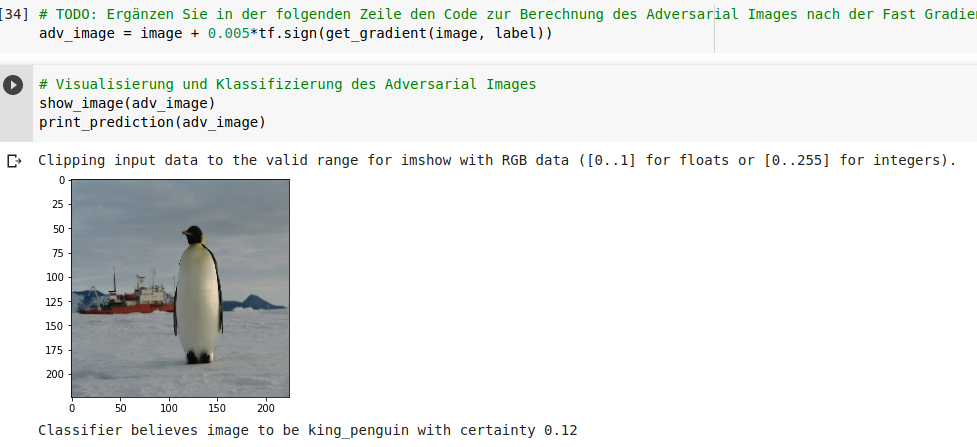
\includegraphics[scale=0.5]{Task4-3_2.png}
\subsection*{Aufgabenteil c}
Der Faktor $\epsilon$ gibt an, wie stark das Originalbild verändert wurde. Ist der Faktor zu hoch, ist das Bild nicht mehr Klassifizierbar, da es sich total verändert hat. Ist der Faktor dahingegen zu niedrig schlägt der Angriff fehl, da sich das Bild kaum merkbar verändert hat.

\subsection*{Aufgabenteil d}
Durch mehrfaches wiederholen einer binären Suche wurde festgestellt, dass der kleinste Wert, der zu einer falschen klassifizerung führte für $\epsilon = 0.002$ war mit einer Wahrscheinlichkeit von 0.4. 

\section*{Vergleich des Carlini-Wagner Angriffs mit der Fast Gradient Sign Methode}
Der Carlini-Wagner Angriff ist im Vergleich zum Fast Gradient Sign Verfahren eine targeted Attacke, wodurch der 
Angreifer bestimmen kann, welche falsche Ausgabe das Modell generieren soll. Dies geht bei dem Fast Gradient Sign Verfahren nicht, dies ist aber schneller, also hat eine kürzere Laufzeit.


\end{document}
